%!TEX root = main.tex
\documentclass[main.tex]{subfiles}

\begin{document}

\chapter{Leveraging pre-trained representations to improve spoken term detection}
\chaptermark{Improving spoken term detection via pre-trained representations}

As recording spoken language is much easier than transcribing the recorded speech, language documentation efforts often yield a substantial amount of untranscribed speech, which is difficult to index and search.~Yet how easily recorded speech can be searched and retrieved has a direct impact on how effectively such resources may be used by all interested parties --- from linguists, to language teachers, to community members.~As introduced in the first chapter, one approach to improve access could be through query-by-example spoken term detection (QbE-STD), which as illustrated in Figure~\ref{fig:qbestd}, enables the use of voice queries to perform searches on untranscribed speech corpora.~Recent work trialling QbE-STD for language documentation corpora have found reduced performance when the speaker of the query was different to those in the corpora.~In this chapter, I examine whether leveraging pre-trained representations can help improve QbE-STD in these scenarios.

\section{Background}

\subsection{What is query-by-example spoken term detection?}

\begin{figure*}[h]
  \centering
  % \vspace{1em}
  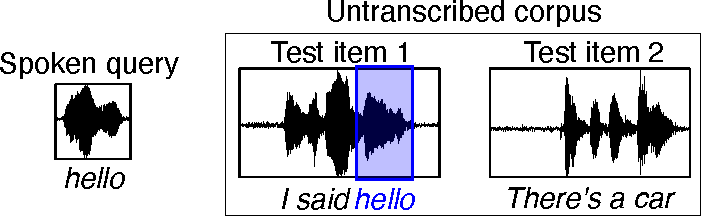
\includegraphics[width=0.4\linewidth]{figures/asru2021-qbestd}
  \caption[An illustration of Query-by-Example Spoken Term Detection]{An illustration of Query-by-Example Spoken Term Detection (QbE-STD)}
  \label{fig:qbestd}
\end{figure*}

\begin{figure*}[t]
  \centering
  % \vspace{1em}
  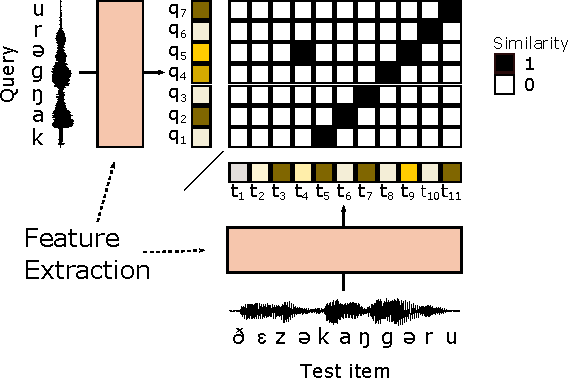
\includegraphics[width=0.55\linewidth]{figures/asru2021-qbestd-stages}
  \caption[An illustration of the feature extraction stage for Query-by-Example Spoken Term Detection]{An illustration of the feature extraction stage for Query-by-Example Spoken Term Detection (QbE-STD)}
  \label{fig:qbestd-feat}
\end{figure*}

In querying a corpus of speech data, we are often interested in finding all instances of a particular spoken form or similar sounding utterances that may constitute minimal pairs --- but how might we accomplish such searches in untranscribed recordings?~Query-by-example spoken term detection (QbE-STD), which, as illustrated in Figure~\ref{fig:qbestd}, is a long-standing speech information retrieval task of finding all regions within a corpus of audio recordings where a spoken query term occurs \parencite{myersInvestigationUseDynamic1980,rohlicek1995Word,fiscusResults2006Spoken2007,rodriguez-fuentesHighperformanceQuerybyexampleSpoken2014}.~In standard terminology, each audio recording in which the spoken query is searched for is considered a `test item'.~A conventional QbE-STD system consists of two broad stages.~In the first stage, information or `features' are extracted from both the query and test items.~The second stage involves calculating a detection score of how likely a query occurs in a test item for each pair of query and test item, typically using a Dynamic Time Warping (DTW) based template matching.

In this chapter, we focus on the feature extraction stage, whose goal is to extract information from the speech signals of the query and test items such that the similarities in their speech content can be compared.~As illustrated in Figure~\ref{fig:qbestd-feat} using a query \emph{kangaroo} [{\fontspec{LinLibertine.ttf}kaŋgəru}] and test item \emph{there’s a \underline{kangaroo}} [{\fontspec{LinLibertine.ttf}ðɛzəkaŋgəru}], the ideal feature extraction process would yield a representation of each that facilitates the correct detection in the second stage.~Roughly summarised, the task of the second stage is to use the representations to look for whether there is a region of high similarity between the query and test item, as illustrated by the diagonal in Figure~\ref{fig:qbestd-feat}.

As is the case for many tasks involving speech, a noise-robust and speaker-invariant feature extraction method is a key component of a performant QbE-STD system.~Indeed, the experiments in \textcite{le-ferrand-etal-2020-enabling} showed that while QbE-STD seemed promising for facilitating searches on speech from language documentation efforts, considerably lower retrieval performance was observed when the speaker of the query and that of the test item were different.~In this chapter, we are interested in whether representations extracted using large-scale pre-trained models are speaker-independent and noise-robust such that they help improve QbE-STD performance for this use case.

\subsection{Related work}

\corr{As mentioned, a spoken term detection system is conventionally composed of two main stages:~feature extraction and detection.~One motivation for focusing on feature extraction is that recent work has shown that for languages without task-specific data to train a neural network based detection system, the conventional, non-neural Dynamic Time Warping (DTW) approach remains extremely competitive.}~For example, recent work has examined using a neural detection system based on a convolutional neural network \parencite[CNN:][]{ramCNNBasedQuery2018} or forgoing conventional stages entirely by using an end-to-end system \parencite{ramNeuralNetworkBased2020}.~However, not all languages benefit equally from these advances.~While the proposed neural systems did outperform the conventional DTW system for larger European languages from the SWS2013 QbE-STD benchmark dataset, the highest performing system for all of the smaller African languages was the conventional DTW system.

\corr{As mentioned, obtaining speaker-independent and noise-robust representations is a critical part of developing a spoken term detection system.~Conventionally, this goal was achieved by training a `bottleneck' feature extractor for phone classification.~That is, the network is designed with an intentional bottleneck which restricts information flow (using a hidden layer that has a lower dimensionality compared to the surrounding layers) and tasked with identifying phones in speech signals.~This design encourages the model to discard information that is irrelevant to phone classification (e.g.~speaker-specific information).}~However, training a bottleneck feature extractor typically requires speech labelled at the phone level, which is costly to generate even for major languages, \corr{restricting their availability to all but the largest of languages.~Given that self-supervised models such as wav2vec 2.0 do not require human labelled data for training, we are interested in discovering whether representations learned in this way are useful for the spoken term detection task, especially for languages for which bottleneck feature extractors are not readily available.}

\corr{Results from \textcite{bartelds2022neural} suggest that representations extracted from a transformer layer of wav2vec 2.0 (w2v2) models may indeed be useful for audio-on-audio comparisons such as spoken term detection.}~Experiments in \textcite{bartelds2022neural} investigated which of the 24 w2v2 Transformer layers may be best suited for automatic pronunciation scoring of non-native English speech.~Similar to QbE-STD, the task of pronunciation scoring is a 2-stage process:~features are extracted from native and non-native speech samples of the same read text, and then a DTW-based distance is calculated (lower distance indicates closer pronunciations).~Results from \textcite{bartelds2022neural} showed that distances between native and non-native speech samples had a strong negative correlation with native speaker ratings of the same samples (\emph{r} = \mbox{-0.85}; lower distances correspond to higher ratings) when computed using representations extracted from the 10th Transformer layer.~In other words, the representations of the middle layers of the w2v2 Transformer network appear to be well-suited for comparing phonetic characteristics of speech samples while being robust to recording conditions and speaker characteristics.

\section{Method}

As mentioned, previous experiments in \textcite{le-ferrand-etal-2020-enabling} trialling QbE-STD with language documentation data showed that occurrences of a query were less likely to be detected when the query and test item being compared were spoken by different speakers.
Our own pilot experiments with Mel-frequency cepstral coefficients (MFCC) and bottleneck features (BNF), which we report here as baselines, had also shown that even when the speaker was the same, acoustic differences arising from recording equipment and/or environment differences can result in similar drops in performance.
Motivated by these issues, we examined whether performance improved with features extracted from various stages of the w2v2 English and multilingual models for QbE-STD using datasets in which the speakers and/or recording conditions between the query and test items were the same, overlapping, or different.
We examined both the English and multilingual w2v2 models as earlier work had shown that for keyword spotting (i.e.~QbE-STD with a closed query set) in West African languages the English w2v model performed on par with a w2v model trained on 10 West African languages \parencite{doumbouya2021usingradio}.

\subsection{Datasets}

\begin{table*}[!b]
  \centering
  \renewcommand{\arraystretch}{1.17}
  \begin{tabular}{llcccc}
    \toprule
    \multirow{2}{*}{Dataset} & \multirow{2}{*}{Language} &  \multirow{2}{*}{\makecell{Number of queries\\(Speakers)}} & \multirow{2}{*}{\makecell{Number of test items\\(Speakers; Duration)}} & \multicolumn{2}{c}{Query vs. Test items} \\ \cmidrule(l){5-5}\cmidrule(l){6-6}
     & & & & Speakers & Recordings \\
    \midrule
    gbb-pd   & Kaytetye         & 397 (1F)     & 397 (1F; 16 mins)   & Same  &  Same  \\
    wrm-pd   & Warumungu        & 383 (1F)     & 383 (1F; 20 mins)   & Same & Same  \\

    
    wrl-mb   & Warlmanpa        & 23  (1F)     & 162 (1F; 11 mins)   & Same & \cellcolor{gray!60}Different  \\
    gup-wat  & Kunwinjku        & 50  (5M)      & 725 (5M, 2F; 32 mins)   & \cellcolor{gray!20}Overlap &  \cellcolor{gray!20}Overlap  \\

    gbb-lg   & Kaytetye         & 189 (1F)     & 809 (8F, 4M; 45 mins)   & \cellcolor{gray!20}Overlap & \cellcolor{gray!60}Different  \\
    
    
    pjt-sw01 & Pitjantjatjara   & 30  (1F)     & 320 (5F; 38 mins)   & \cellcolor{gray!60}Different & \cellcolor{gray!60}Different  \\
    mwf-jm   & Murrinhpatha     & 37  (1F, 1M) & 259 (3F, 2M; 13 mins)   & \cellcolor{gray!60}Different & \cellcolor{gray!60}Different  \\
    wbp-jk   & Warlpiri         & 24  (1F)     & 198 (12F; 6 mins)    & \cellcolor{gray!60}Different & \cellcolor{gray!60}Different  \\
    

    \cmidrule(lr){1-6}
    gos-kdl  & Gronings         & 83 (2F, 3M)           & 430 (2F, 2M; 23 mins)   & \cellcolor{gray!20}Overlap & \cellcolor{gray!20}Overlap  \\
    eng-mav  & English          & 100 (1M)     & 526 (1M; 77 mins)   & \cellcolor{gray!60}Different & \cellcolor{gray!60}Different  \\
    \bottomrule
  \end{tabular}
  \caption[Characteristics of evaluation datasets used for spoken term detection.]{Characteristics of evaluation datasets. Parentheticals indicate speaker compositions, and total length of test audio in minutes. Same, overlap, or different indicate whether the queries and test items shared speakers and/or recording conditions.}
  \label{tab:datasets}  
\end{table*}

We curated data from English, Gronings, and 7 Australian Aboriginal languages.~Gronings and all of the Australian languages are currently classified as vulnerable or endangered \parencite{eberhard_ethnologue_2020}.~For these languages, the audio were sourced from various language documentation projects (e.g., audio for dictionaries, audio book of short stories) and thus constitute in-domain test data for the QbE-STD systems evaluated.

We gathered for each language queries from 1-5 speakers consisting of words and multi-word expressions and test items consisting of longer utterances from 1-12 speakers.
Each dataset varied according to whether the query and test items shared speaker(s) and/or recording conditions, as indicated in Table \ref{tab:datasets}.
For example, for gbb-lg, the 189 queries were sourced from audio produced in a recording studio by a single female speaker AR.
The 809 test items were sourced from various field recordings from 12 speakers (8F, 4M: one of whom was AR).
Thus, for gbb-lg, the queries and test items overlapped in speakers but differed in recording conditions.

\subsection{Pre-trained models}

In our feature extraction procedure, we use two w2v2-based models, namely the English monolingual model described in \textcite{NEURIPS2020_92d1e1eb} and the multilingual `XLSR53' model described in \textcite{conneau21_interspeech}.
The English monolingual model is pre-trained on the unlabelled Librispeech dataset (LS960), which contains 960 hours of clean and noisy English speech from audio books.
The multilingual model is pre-trained on 56,000 hours of data from 53 different languages (amount of data varies per language, though 44,000 hours of English from the Multilingual Librispeech dataset constitutes the majority), and includes African, Asian, and European languages obtained from audio books, conversational telephone speech, and read speech.
% Due to the larger amount of languages, the XLSR53 model might have learned speech representations that are useful for modelling the languages in our endangered language dataset.
The architecture of both models is the same, except for the quantisation of the encoder representations.
XLSR53 learns a single set of quantised speech representations on the basis of the encoder output.
This set was subsequently shared across languages, which was shown to be effective for learning self-supervised multilingual speech representations for ASR.

\subsection{Procedure}

To create ground truth labels, we first paired each query's text transcription with that of each test item within a given dataset.~Then for each pair, we used regular expressions to determine whether the query occurred in the test item.~All audio data from various sources were standardised to mono 16-bit PCM at 16 kHz (sample rate required by w2v2).~For MFCC and bottleneck features (BNF), the audio was further downsampled to 8 kHz at extraction time to meet the requirements of the respective feature extractors.

For baseline comparisons, we extracted MFCC and BNF representations using the Shennong library,\footnote{https://docs.cognitive-ml.fr/shennong/} which provides a Python interface to common feature extraction routines.~For MFCC, we used the Kaldi feature extractor which returns for each time frame 13 MFCC features with their first and second derivatives (39 features total).~For BNF, we used the BUT/Phonexia feature extractor which returns for each time frame 80 activation values from a bottleneck layer originally trained for phone classification on the 17 languages of the IARPA Babel dataset \parencite{silnovaPhonexiaBottleneckFeature2018}.~For w2v2 features (both from the English monolingual model and XLSR53 multilingual model), we adapted the feature extraction code from \textcite{bartelds2022neural},\footnote{https://github.com/Bartelds/neural-acoustic-distance} which extracts outputs from the Encoder CNN (E), the Quantiser module (Q), or any one of the 24 layers of the Transformer network (T01--T24).
Thus, in total we extracted features using 54 different methods for each of the 10 datasets.

As our primary interest is in comparing different feature extraction methods, we implemented a DTW-based detection stage based on a state-of-the-art QbE-STD system \parencite{rodriguez-fuentesHighperformanceQuerybyexampleSpoken2014}.~Given two feature matrices, of a query $Q$ and of a test item $T$, we calculated standardised Euclidean distances between each time frame in $Q$ and $T$.~To make distances between different pairs of queries and test items comparable, these distances were range normalised to [0, 1].~A window the size of the query was moved along the normalised distance matrix and a DTW-based distance between the query and subpart of the test item was calculated at each step.~The score for how likely a query occurs in a test item was then calculated as 1 minus the minimum distance.

We used the Maximum Term Weighted Value (MTWV) to evaluate each of our QbE-STD systems (e.g. MFCC+DTW, w2v2-E+DTW, etc.).~The MTWV ranges from 0, indicating a system that simply returns nothing, to 1, indicating a perfect system detecting all relevant instances with no false positives.~Using the NIST STDEval tool,\footnote{https://www.nist.gov/itl/iad/mig/tools} we calculated MTWVs with the suggested NIST costs (false positive: 1, false negative: 10) and an empirical prior of 0.0278 (true positive rate averaged across all 10 datasets).~With these costs, a MTWV of 0.48 indicates a system that correctly detects 48\% of all queries searched,\footnote{\corr{To the best of my knowledge, there have not been user studies examining the relationship between MTWV and usability of a spoken term detection system (e.g.~analogous to those in automatic speech recognition and the word error rate metric).}} while producing at most 10 false positives for each true positive correctly retrieved \parencite{whiteUsingZeroresourceSpoken2015}.

For significance testing, we computed the MTWV for each query in a given dataset and performed a one-sided paired \emph{t}-test to examine whether the MTWVs obtained for the queries using one feature extraction method were significantly greater than those obtained using another method.

With the exception of the raw audio and transcriptions from the Australian language documentation projects for which we do not have permissions to release openly, we have made all pilot experiments results, experiment code and analyses available on a GitHub repository, and placed the Gronings data and all experimental artefacts in Zenodo archives.\footnote{All linked on: https://github.com/fauxneticien/qbe-std\_feats\_eval\label{ghlink}}
The English data can be obtained from the Mavir corpus \parencite{sandoval2012mavir}.\footnote{http://www.lllf.uam.es/ING/CorpusMavir.html}

\section{Results and discussion}

\corr{Figure \ref{fig:mtwv} displays spoken term detection performance as measured by MTWV (y-axis; higher is better), and how this performance varies across the 10 datasets (indicated by shapes) and various feature extraction methods (x-axis:~MFCC, BNF), including those extracted from various layers (E, Q, T01, ..., T24) from two wav2vec 2.0 models (LS960, trained only on English; XLSR53, trained on 53 languages).}~As expected, dataset characteristics had a clear effect on QbE-STD performance.~For our baselines, retrieval performance using MFCC was highest on the datasets having the same speaker and recordings between the queries and test items (wrm-pd: 0.83; gbb-pd: 0.71), lower on those with overlapping speakers (e.g.~wrl-mb: 0.48) or recordings (e.g.~gup-wat: 0.33), and lowest when both were entirely different (e.g.~wbp-jk: 0.18, mwf-jm: 0.14).~The same effects were also seen using BNF, which improved on different-speaker/recordings datasets (e.g.~wbp-jk: 0.27), though at the cost of worsening on those with same-speaker/recordings (e.g.~wrm-pd: 0.71).

\begin{figure}[!t]
  \centering
  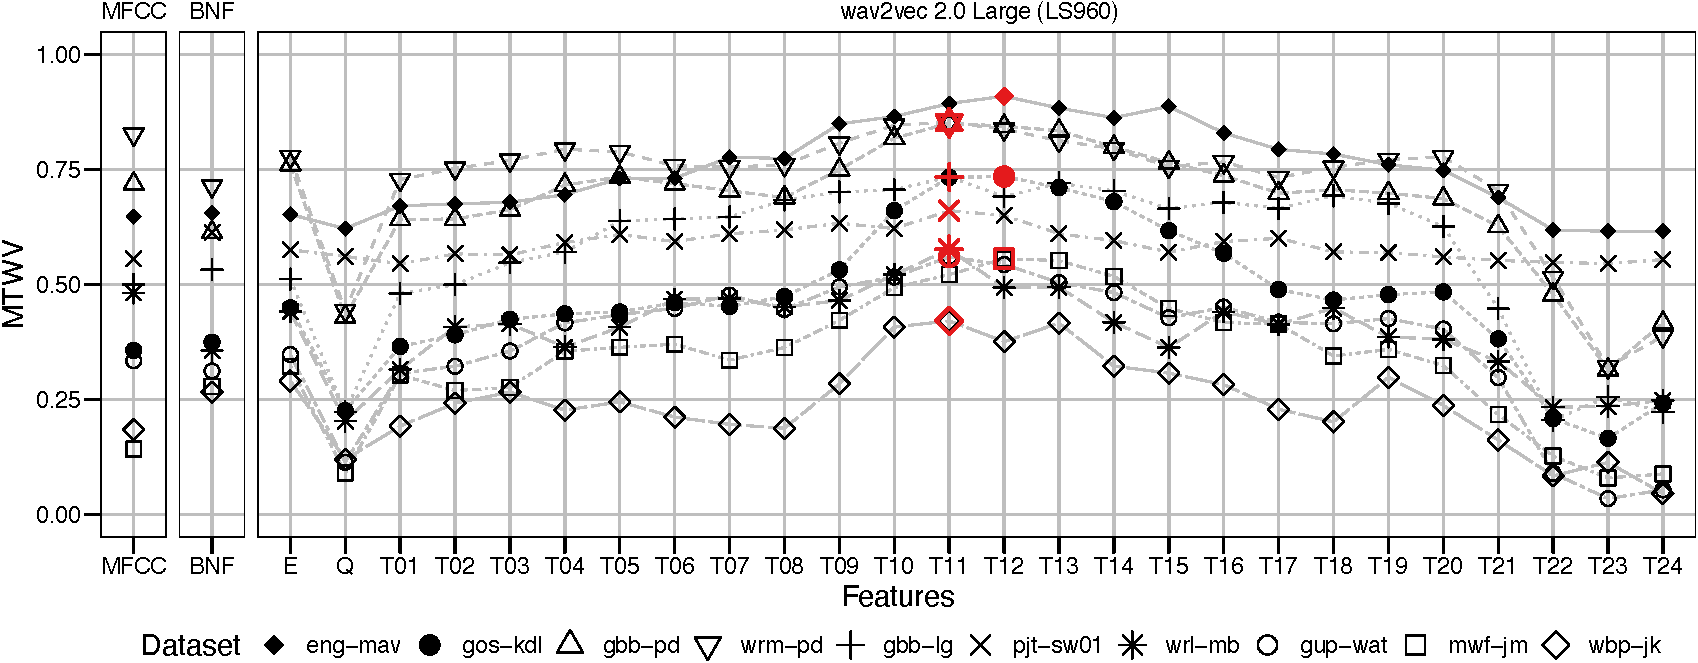
\includegraphics[width=1.0\linewidth]{figures/asru2021-ls960-layers}
  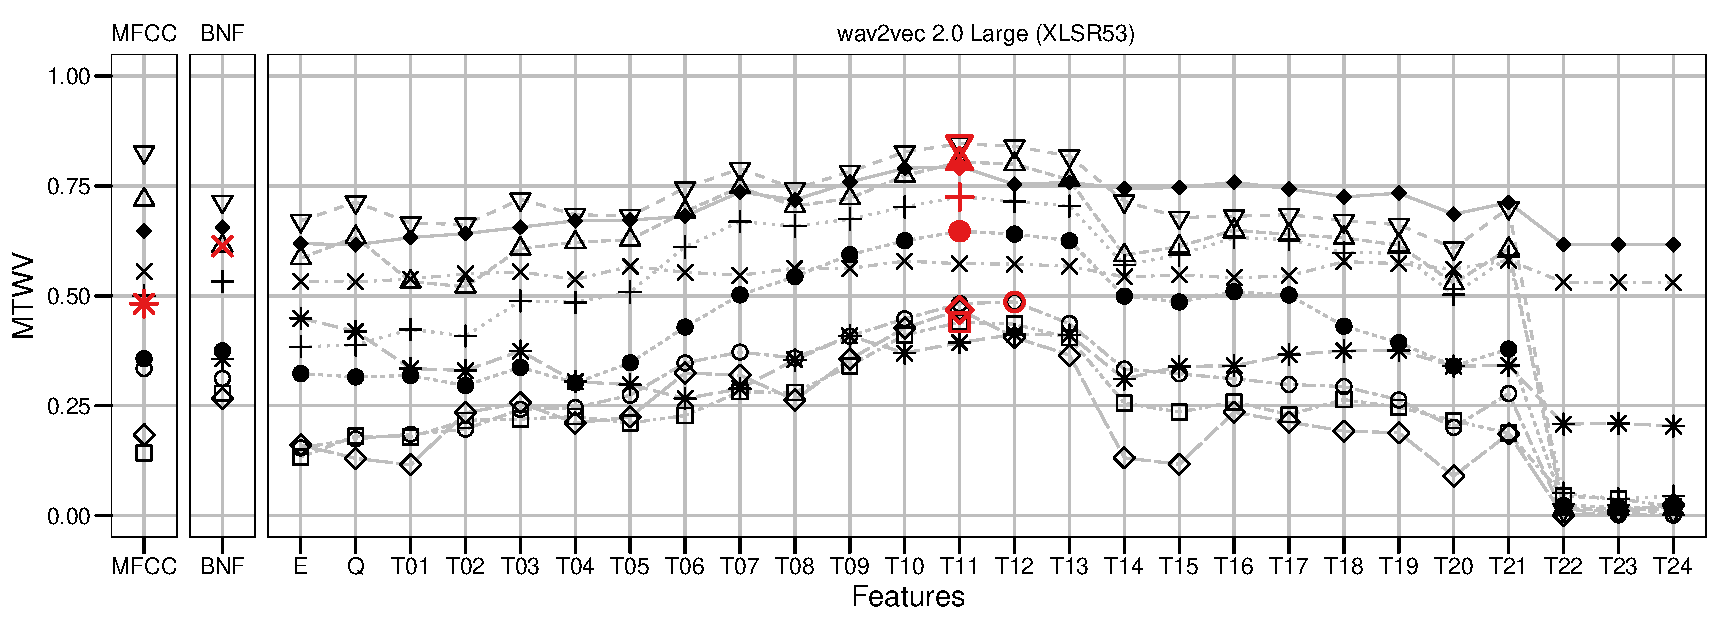
\includegraphics[width=1.0\linewidth]{figures/asru2021-xlsr53-layers}
  \caption[Query-by-Example Spoken Term Detection results leveraging wav2vec 2.0 models for feature extraction]{Maximum Term Weighted Values achieved on a QbE-STD task using various speech representations: baselines (MFCC; bottleneck features: BNF) and from layers (E; Q; T01-24) of two wav2vec 2.0 models (English monolingual: LS960; multilingual: XLSR53).~Shapes indicate one of 10 datasets; red-coloured/largest shape indicates highest score achieved on dataset.}
  \label{fig:mtwv}
\end{figure}

\begin{table*}[!ht]
  \centering
  \renewcommand{\arraystretch}{1.1}
  \scalebox{0.9}{\begin{tabular}{lccccccc}
      \toprule
      \multirow{2}{*}{\makecell{Dataset\\($N$ queries)}} & \multicolumn{3}{c}{MTWV (averaged over queries)} & \multicolumn{3}{c}{One-sided paired \emph{t}-test (\emph{t}-value, \emph{p}-value)} \\ \cmidrule(l){2-4}\cmidrule(l){5-7}
       & a. BNF & b. LS960-T11 & c. XLSR53-T11 & $H_1$: b. $>$ a. & $H_1$: c. $>$ a. & $H_1$: b. $>$ c. \\
      \midrule
      gbb-pd (397)   & 0.612         & 0.849     & 0.803   & (14.1, .000)  &  (11.1, .000) & (3.8, .000) \\
      wrm-pd (383)  & 0.713        & 0.853     & 0.843   & (8.7, .000) & (8.2, .000) & \cellcolor{gray!60}(0.7, .236) \\
      wrl-mb (23) & 0.352        & 0.573     & 0.379   & (3.0, .003) & \cellcolor{gray!60}(0.3, .372) & (3.4, .001) \\
      gup-wat (50) & 0.313        & 0.561      & 0.483   & (6.6, .000) &  (3.9, .000) & (2.7, .005) \\
      gbb-lg (189) & 0.533         & 0.733     & 0.719   & (6.7, .000) & (6.6, .000) & \cellcolor{gray!60}(0.5, .299) \\
      pjt-sw01 (30) & 0.607   & 0.660     & 0.572   & \cellcolor{gray!60}(1.4, .080) & \cellcolor{gray!60}(-0.9, .082) & (2.2, .020)  \\
      mwf-jm (37) & 0.279     & 0.515 & 0.435   & (4.8, .000) & (2.4, .010) & \cellcolor{gray!60}(1.3, .102) \\
      wbp-jk (24) & 0.267         & 0.422     & 0.468   & (1.9, .037) & (2.6, .009) & \cellcolor{gray!60}(-0.6, .732)  \\
      \cmidrule(lr){1-7}
      gos-kdl (83) & 0.372         & 0.728           & 0.647   & (9.8, .000) & (8.2, .000) & (2.9, .002) \\
      eng-mav (100) & 0.656          & 0.894     & 0.794   & (11.1, .000) & (5.7, .000) & (3.9, .000)  \\
      \bottomrule
    \end{tabular}}
    \caption[Results of spoken term detection evaluations]{Results of one-sided \emph{t}-tests for the alternative hypothesis ($H_1$) that the Maximum Term Weighted Value (MTWV) obtained for each query in a given dataset is greater using different speech representations: baseline bottleneck features (BNF), and Transformer layer 11 (T11) of two wav2vec 2.0 models (English monolingual: LS960; multilingual: XLSR53).}
  \label{tab:ttests}
  \vspace{-1em}
\end{table*}

Using outputs from a middle Transformer layer of a w2v2 model resulted in increased performance on nearly all our datasets.~For 9 of 10 datasets, the MTWVs obtained using outputs of the Transformer layer 11 from the English monolingual model were significantly greater than those obtained using BNF, as indicated by the $t$-tests in Table \ref{tab:ttests} (b. LS960-T11 $>$ a. BNF).~Similarly, the MTWVs obtained using Transformer layer 11 of the multilingual model were significantly greater than those using BNF for 8 of 10 datasets (Table \ref{tab:ttests}: c. XLSR53-T11 $>$ a. BNF).~Overall, the best performing representations were those from the Transformer layer 11 of the English w2v2 model, which also significantly outperformed those from the equivalent layer of the multilingual w2v2 model for 4 of the 8 Australian language datasets (Table \ref{tab:ttests}: b. LS960-T11 $>$ c. XLSR53-T11).~On the two most challenging Australian language datasets with different speakers and recordings, performance increased 56-86\% using T11 features of the English model (wbp-jk: 0.42, mwf-jm: 0.52) over the best achievable baseline scores using BNF (wbp-jk: 0.27, mwf-jm: 0.28); n.b. the English and multilingual models did not differ significantly on these two datasets.~These results demonstrate the effectiveness of contextualised representations learned by the Transformer network for comparing the phonetic characteristics of speech samples while being robust to recording conditions and speaker characteristics.

To better understand the representations of the Transformer layer 11 of the English w2v2 model, we undertook an error analysis of the erroneous retrievals by the QbE-STD system on the Australian languages when using these features.We focused on `unretrievable' queries, defined as those for which no true matches were present in the top 5 results returned for that query, and examined the differences in phonetic transcriptions between the query and its top match.~This analysis revealed that for the majority of these queries (89/119 = 75\%), there were 4 or fewer segmental differences between the transcriptions of the query and its top match, and that, notably, the query and its top match typically shared a manner template.~For example, for the Kaytetye query [{\fontspec{LinLibertine.ttf}aɳanpə}] `medicinal sap', its top match was the word [{\fontspec{LinLibertine.ttf}anənkə}] `to sit', both of which share the VNVNTV template (where V represents a vowel, N a nasal, and T a plosive).~In other words, the representations of the w2v2 English model do not appear to be sufficiently fine-grained to differentiate between segments differing primarily in place of articulation, especially for those that do not occur contrastively in English (e.g. retroflex nasal [{\fontspec{LinLibertine.ttf}ɳ}] vs. alveolar nasal [{\fontspec{LinLibertine.ttf}n}]).\footnote{\corr{For an experimental investigation of comparing how native and non-native speech perception patterns in humans compare with in- and out-of-domain languages for self-supervised speech models see \textcite{millet2022self,millet2022predicting}}}

\subsection{Exploring wav2vec 2.0 features}

\begin{figure*}[t]
  \vspace{1em}
  \centering
  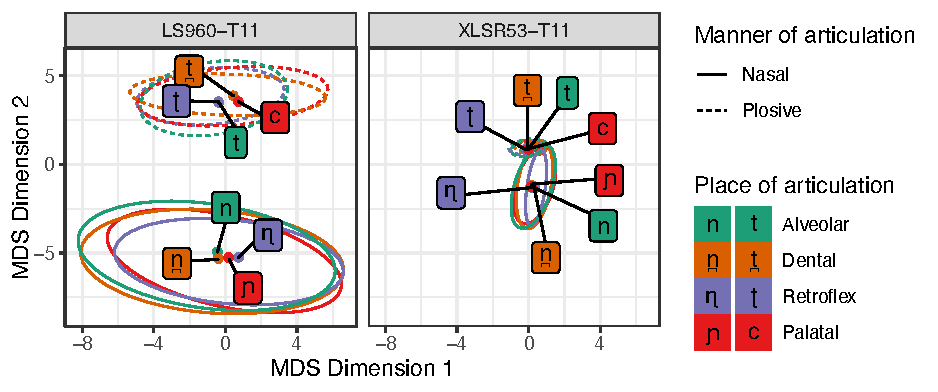
\includegraphics[width=0.8\linewidth]{figures/asru2021-ellipses}
  \caption[Visualisations of features extracted using wav2vec 2.0 models]{Multidimensional scaling (MDS) visualisations of features extracted from Kaytetye consonants (data from \cite{harvey2015contrastive}) using Transformer layer 11 (T11) of wav2vec 2.0 (English monolingual: LS960; multilingual: XLSR53), averaged over the duration of the consonant. Ellipses represent 95\% confidence intervals and text labels represent means.}
  \label{fig:ellipses}
  % \vspace{-1em}
\end{figure*}

Based on the findings of our error analysis, we examined whether differences in the way phonetic information is encoded by the w2v2 English and the multilingual models could explain differences in their QbE-STD performance.~We used the Transformer layer 11 of the English and multilingual models to extract features from Kaytetye consonants (from audio stimuli collected by \cite{harvey2015contrastive}).~Figure \ref{fig:ellipses} displays the dissimilarities between each of the Kaytetye consonant types in the 1024-dimensional space of the two w2v2 models (averaged across the duration of the consonant and reduced to 2 dimensions through multidimensional scaling).~For considerations of space and visual clarity, we focus on the nasals and plosives.

Despite being given no phone labels at training time, the w2v2 models learn to encode broad manner of articulation classes within its representations, as evidenced by ellipses forming two clusters for nasals (solid lines) and plosives (dashed lines) in Figure \ref{fig:ellipses}.~In line with findings from our qualitative error analysis, features from the w2v2 English model under-differentiate place of articulation contrasts, as evidenced by the overlapping ellipses within each of the nasal and plosive manners of articulation in Figure \ref{fig:ellipses}.~Compared to the English model, the representations of the Kaytetye consonants by the multilingual model overlap to a larger degree.~This result suggests that representations extracted from a model trained on a single language or a set of phonologically similar languages may be more beneficial for QbE-STD than a large multilingual model such as XLSR53 trained on a diverse set of 53 languages --- especially when supervised fine-tuning in the target languages is not a readily available option.

\section{Conclusion}

In this chapter, we compared the performance of 54 feature extraction methods for QbE-STD using data from 9 languages, eight of which are vulnerable or endangered.~Our results showed that the middle layers of the wav2vec 2.0 Transformer network provide a noise-robust and speaker-invariant representation of speech sounds that can be leveraged for QbE-STD with low resource languages, performing significantly better than state-of-the-art approaches using bottleneck features.~An error analysis and a preliminary investigation of the information encoded in the representations learned by the wav2vec 2.0 Transformer network suggested that the representations extracted from the English model may provide better features for QbE-STD in unrelated languages than the multilingual model in cases where important phonological distinctions in those languages are not as distinctively encoded by the multilingual model.~Given the alternative is browsing untranscribed audio in near real-time, QbE-STD does help provide better access via enabling voice searches.~However, the inherent difficulty of an audio-on-audio the matching task may limit its capabilities, especially on noisy field recordings in archival corpora.

\end{document}
